% -*- latex -*-
%%%%%%%%%%%%%%%%%%%%%%%%%%%%%%%%%%%%%%%%%%%%%%%%%%%%%%%%%%%%%%%%
%%%%
%%%% This TeX file is part of the course
%%%% Introduction to Scientific Programming in C++/Fortran2003
%%%% copyright 2017-9 Victor Eijkhout eijkhout@tacc.utexas.edu
%%%%
%%%% struct.tex : about structures
%%%%
%%%%%%%%%%%%%%%%%%%%%%%%%%%%%%%%%%%%%%%%%%%%%%%%%%%%%%%%%%%%%%%%

\Level 0 {Why structures?}
\label{sec:struct}

You have seen the basic datatypes in section~\ref{sec:ctypes}. These
are enough to program whatever you want, but it would be nice if the
language had some datatypes that are more abstract, closer to the
terms in which you think about your application. For instance, if you
are programming something to do with geometry, you had rather talk
about points than explicitly having to manipulate their coordinates.

Structures are a
first way to define your own datatypes. A~\indextermttdef{struct}
acts like a datatype for which you choose the name. A~\lstinline$struct$
contains other datatypes; these can be elementary, or other structs.
%
\verbatimsnippet{structdef}

The elements of a structure are also called
\emph{members}\index{member!of struct}.
You can give them an initial value:
\begin{lstlisting}
struct vector { double x=0.; double y=0.; } ;
\end{lstlisting}
  
\begin{slide}{Bundling information}
  \label{sl:struct-why}
  Sometimes a number of variables belong logically together. For
  instance two doubles can be the $x,y$ components of a vector.

  This can be captured in the \lstinline$struct$ construct.

  \verbatimsnippet{structdef}

  (This can go in the main program or before it.)

The elements of a structure are usually called \indexterm{members}.
\end{slide}

\Level 0 {The basics of structures}

A structure behaves like a data type: you declare variables of the
structure type, and you use them in your program. The new aspect is
that you first need to define the structure type. This definition can
be done inside your main program or before it. The latter is
preferable, for instance if you need to pass the structure to a function.

\begin{lstlisting}
// definition of the struct
struct AStructName { int num; double val; }
int main() {
  // declaration of struct variables
  AStructName mystruct1,mystruct2;
  .... code that uses your structures ....
}
\end{lstlisting}

\begin{slide}{How to use structures}
  \label{sl:structinprog}
  \begin{enumerate}
  \item Declare what is in your structure;
  \item Make some structures;
  \item Use them.
  \end{enumerate}
\begin{lstlisting}
// definition of the struct
struct AStructName { int num; double val; }
int main() {
  // declaration of struct variables
  AStructName mystruct1,mystruct2;
  .... code that uses your structures ....
}
\end{lstlisting}
\end{slide}

There are various ways of setting the members of the structure:
\begin{itemize}
\item You can set defaults that hold for any structure of that type;
\item you can all members at once;
\item or you can set any member individually.
\end{itemize}

\begin{block}{Struct initialization}
  \label{sl:structinit}
  You assign a whole struct, or set defaults in the definition.
  %
  \verbatimsnippet{pointinit}
\end{block}

\begin{block}{Using structures}
  \label{sl:struct-use}
  Once you have defined a structure, you can make variables of that
  type. Setting and initializing them takes a new syntax:
  %
  \snippetwithoutput{structuse}{struct}{point}
  %
  Period syntax: `apostrophe-s'.
\end{block}

\begin{exercise}{Quick review}
  \label{rev:func-def}
  True or false?
  \begin{itemize}
  \item All members of a struct have to have the same type.
  \item Writing
\begin{lstlisting}
struct numbered { int n; double x; };
\end{lstlisting}
creates an object with an integer and a double as members.
\item With the above definition and \lstinline$struct numbered xn;$,
\begin{lstlisting}
cout << xn << endl;
\end{lstlisting}
is correct C++.
\item Same, 
\begin{lstlisting}
xn.x = xn.n+1;
\end{lstlisting}
  \end{itemize}
\end{exercise}

Note: if you use initializations in the \lstinline$struct$ definition,
you can not use the brace-assignment.

\begin{block}{Functions on structures}
  \label{sl:struct-pass}
  You can pass a structure to a function:
  %\verbatimsnippet{structpass}
  \snippetwithoutput{structpass}{struct}{pointfun}
\end{block}

\begin{exercise}
  \label{ex:vecstruct-angle}
  \hbox{%
    \begin{minipage}[t]{.6\hsize}
      Write a function that, given a vector as defined above, returns the
      angle with the $x$-axis. (Hint: the \lstinline$atan$ function is in \lstinline$cmath$)
    \end{minipage}
    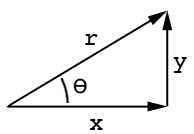
\includegraphics[scale=.4]{xy-atan}
    }

  \answerwithoutput{anglepi4}{struct}{pointangle}
\end{exercise}

\begin{exercise}
  \label{ex:vecstruct-flip}
  Write a \lstinline$void$ function that has a \lstinline$struct vector$ parameter,
  and exchanges its coordinates:
  \[ \begin{pmatrix}2.5\\3.5\end{pmatrix} \rightarrow
    \begin{pmatrix}3.5\\2.5\end{pmatrix} \]
  \answerwithoutput{flip32}{struct}{pointflip}
\end{exercise}

\begin{exercise}
  \label{ex:vecstruct-scale}
  Write a function $y=f(x,a)$ that takes a \lstinline$struct vector$ and
  \lstinline$double$ parameter as input, and returns a vector that is the
  input multiplied by the scalar.
  \[ \begin{pmatrix}2.5\\3.5\end{pmatrix},3 \rightarrow
    \begin{pmatrix}7.5\\10.5\end{pmatrix} \]
\end{exercise}

\begin{exercise}
  \label{ex:primestruct}
  If you are doing the prime project (chapter~\ref{ch:prime}) you can
  now do exercise~\ref{ex:prime:struct}.
\end{exercise}

\begin{exercise}
  \label{ex:vecstruct}
  Write a function \lstinline$inner_product$ that takes two \lstinline$vector$
  structures and computes the inner product.
\end{exercise}

\begin{block}{Denotations}
  \label{sl:struct-denote}
  You can use initializer lists as struct
  \emph{denotations}\index{struct!denotation}:
  %
  \snippetwithoutput{structdenote}{struct}{pointdenote}
\end{block}

\begin{exercise}
  \label{ex:struct-denote}
  Take exercise \ref{ex:vecstruct} and rewrite it to use denotations.
\end{exercise}

\begin{block}{Returning structures}
  \label{sl:struct-return}
  You can return a structure from a function:
  %
  \snippetwithoutput{structreturn}{struct}{pointadd}

  (In case you're wondering about scopes and lifetimes here: the
  explanation is that the returned value is copied.)
\end{block}

\begin{exercise}
  \label{ex:matstruct}
  Write a $2\times 2$ matrix class (that is, a structure storing 4
  real numbers), and write a function \lstinline$multiply$
  that multiplies a matrix times a vector.

  Can you make a matrix structure that is based on the vector
  structure, for instance using vectors to store the matrix rows, and
  then using the inner product method to multiply matrices?
\end{exercise}

\begin{block}{Passing structures by reference}
  \label{sl:struct-passref}
  Prevent copying cost by passing by reference, use \lstinline$const$ to
  prevent changes:
  \verbatimsnippet{structpassref}
\end{block}



